\documentclass[10pt,psfig,letterpaper,twocolumn]{article}
\usepackage{geometry}
\usepackage{graphicx}
\usepackage{setspace}
\usepackage{mdwlist}
\usepackage{natbib}
\usepackage{hyperref}
\usepackage{har2nat}
%\usepackage{named}
%\usepackage[super,sort]{natbib}
%\usepackage[numbers,sort&compress]{natbib}

%\renewcommand{\rmdefault}{ptm}
%\renewcommand{\bfdefault}{b}
%\usepackage{helvet}
\usepackage[scaled=0.9]{helvet}
%\usepackage{courier}
%\normalfont % in case the EC fonts aren't available
%\usepackage[T1]{fontenc}

%\usepackage{multicol}
%\usepackage{doc}
%\usepackage{float}

%\newcommand\bibname{\small{REFERENCES}}
\singlespacing
\paperwidth 8.5in
\paperheight 11in
\oddsidemargin 0in
%\oddsidemargin -0.25in
%\topskip 0in
%\topsep 0in
\headsep 1.3cm 
%\headsep 6mm 
%\headheight 0in 
%\topmargin 0in
%\topmargin -0.25in
%\topmargin -0.85in
\geometry{left=0.75in,top=0.75in,right=0.75in,bottom=1in}
%\evensidemargin 
\textwidth 7in 
\textheight 9.25in
\columnsep 0.4in
%\headheight 0cm
%\footheight 1cm
\footskip 0in 
%\partopsep -0.5cm
%\textfloatsep 0.3cm
%\intextsep 0.3cm

%\makeatletter
%\newenvironment{tablehere}{\def\@captype{table*}}{}

%\newenvironment{figurehere}
%  {\def\@captype{figure}}
%  {}
%\makeatother
\renewcommand{\bibname}{REFERENCE}
\pagestyle{empty} 
\begin{document}
%\bibliographystyle{named} 
%\include{ref}


%\pagestyle{plain} 
%\def\Try#1#2{{\fontfamily{#1}\selectfont}}
\title{\fontfamily{phv}\selectfont{\huge{\bfseries{Crowd-sourcing Invasive Alien Species data}}}}
\author{
{\fontfamily{ptm}\selectfont{\large{\bfseries{Stephen Pike}}}}\thanks{... email: steve@synfinity.net }, \and
{\fontfamily{ptm}\selectfont{\large{\bfseries{Daniel Jones}}}}\thanks{Swansea University. email: 606373@swansea.ac.uk}, \and 
{\fontfamily{ptm}\selectfont{\large{\bfseries{Martin Allison}}}}\thanks{Potato, Bristol. email: martin.allison@potatolondon.com}, \and
{\fontfamily{ptm}\selectfont{\large{\bfseries{Mark Allison}}}}\thanks{... email: mallison77@gmail.com}\\
}
\date{}
\maketitle
\thispagestyle{empty}
\begin{abstract}
Invasive Alien Species (IAS) are a growing global problem, reducing biodiversity and causing significant negative socioeconomic impacts. Management and control is hampered by a lack of accessible data of adequate spatial and temporal resolution. Smart phone technology and cheap access to data networks may enable crowd-sourcing of IAS data to bridge the `data gap'. By engaging the general public in `citizen science', IAS-ESS (iAssess) aims to provide much-needed, real-time data to scientists.
\end{abstract}
{\bf Keywords:}
Citizen science; Crowd-sourcing; Invasive Alien Species (IAS);  Public engagement; Smart phones.
\section*{\fontfamily{phv}\selectfont{\normalsize{\bfseries{Introduction}}}}

Invasive Alien Species (IAS) are an increasing global problem with multiple negative impacts upon biodiversity and socioeconomic interests \cite{Pimentel:2005p4121, Vila:2011ft, Vitousek:1997p78}. Though the effects of IAS have been recognised for decades, management and/or control has been hampered by the lack of accessible data of adequate spatial and temporal resolution  \cite{Vitousek:1997p78}.

Mobile computing and `citizen science' has expanded markedly in recent years \cite{Silvertown:2009tw}. Use of mobile computer technologies, in combination with enhanced Internet service provision, enables rapid acquisition of data from millions of people (known as `crowd-sourcing' \cite{Wired:2011uj}); the world can be perceived as a network of human sensors \cite{Goodchild:2007vt}. In \citet{Hart:2006uz}, Environmental Sensor Networks (ENS) are described as:

\begin{quote}\em{\footnotesize
[comprising of] an array of sensor nodes and a communications system which allows their data to reach a server...
}
\end{quote}

It is clear that one can include the human sensor network in this classification, and indeed, citizen science should be embraced in this manner.

\subsection*{\fontfamily{phv}\selectfont{\normalsize{Related work}}}
Whilst other species sighting/recording services exist\footnote{\url{http://www.brc.ac.uk/}}\footnote{\url{http://www.ispot.org.uk/}}\footnote{\url{http://nonnativespecies.org}}, iAssess is dedicated to the monitoring of IAS.
Functionally and aesthetically, \citet{ispot} is a superb modern website for the logging and identification of \emph{any} species.
It enables the hobbyist to keep track of their sightings, and contribute to a body of phenological data; and enables the novice to gain confidence in identification and appreciation for the natural world.

\citet{nonnativespecies} on the other hand is geared toward identification information about IAS, and allows logging of sightings (via Recording Invasive Species Counts (RISC)),
yet does not allow the IAS scientist to quickly and easily add their professional interest,
and thus leverage the existing user-community.
\citet{nonnativespecies} do encourage users to submit sightings of other IAS, but via an email address, thus in an un-structured way, with the onus on the user to do the hard work.



\section*{\fontfamily{phv}\selectfont{\normalsize{\bfseries{Objectives}}}}

The aims of the iAssess website are:
\begin{enumerate*}
\item Facilitate Invasive Alien Species scientists in the mass-collection of sighting data.
\item Facilitate citizen scientists in contributing to Invasive Alien Species science.
\item Enable Invasive Alien Species management teams to easily establish changing priorities.
\item Produce appealing data visualisations (primarily using geo-location data) to engage the public.
\item As a consequence of increase public engagement, increase awareness of the problems of Invasive Alien Species.
\end{enumerate*}

\section*{\fontfamily{phv}\selectfont{\normalsize{\bfseries{Public Engagement, Citizen Science \& Crowdsourcing}}}}

\citet{Dickinson:2010ug} discuss the various merits of citizen science, and with reference to IAS conclude that ``new tools for merging biodiversity databases would facilitate integrated research on ecological invasions''.
They also identify and review flaws in citizen-science data, including problems in spatial sampling effort --
a factor which may affect iAssess due to reliance on Internet connectivity in mobile applications.

\citet{Wightman:2010un} analysed various crowd-sourcing websites and crucially, find that those who contribute to a crowd-source task are motivated more by the task itself than any reward.
Also, they find that the simpler the task is to perform, the more likely it is to be performed even if it is of low importance to the user.
Although perhaps obvious, these findings remain crucial to engaging the public for scientifically important endeavours such as the monitoring of IAS.
Thus, iAssess requires minimal setup and privacy concern for the casual user to be able to add their data; there is no sign up process, and the mobile software available is free to download and use.

Whilst crowd-sourced data gathering by citizen scientists is clearly valuable to academics and the professional scientific community,
there remains a problem with data validity and unintended consequences of mis-information.
\citet{Schenk:2009ud} note that one cannot control one's crowd,
and it is likely to contain both experts and novices
(indeed, the authors posit further that it will contain a high noise to signal ratio, also!)

In \citet{Somaweera:2010vi}, the authors find that attempts by the public to control the Cane toad (\emph{Bufo marinus}) are often at a cost to the other native anurans, where identification is not sound.
\citet{Somaweera:2010vi} find that community groups and awareness programs reduce mis-identification.
In iAssess a `validation' system is used to show only those sightings that have been verified by an expert, and these can later be used to feed back to users wishing to perform their own identification.
Indeed, a gallery of each taxon is available, with an interactive map -- a sighting made in a particular location where others have already been validated should invoke confidence and persistence in users.
With the focus being firmly on sighting and logging, with data for use by management experts, the propensity toward taking personal action against IAS should be reduced. 

While \citet{GarciaLlorente:vx} note that people are more willing to pay for removal rather than prevention of IAS, \citet{Sharp:2011eh} find that removal of IAS can be viewed unfavourably by the public.
This is particularly the case where removal is through toxic or destructive processes, and that public engagement is crucial to ameliorating the resistance to this activity.
\citet{GarciaLlorente:vx} also found that individuals' opinions of the practice are influenced by their knowledege and understanding of the IAS and its affects.
By encouraging the public to partake in the sighting and reporting of IAS, it is hoped that they will feel more comfortable during the subsequent removal/management of the species;
particularly if they feel like they have contributed positively. 

Aside from the perceptions of the public on the management of IAS,
there has been argument \cite{Brown:2004uj} for dispassionate study of IAS,
followed by counter-argument \cite{Larson:2007vs} in favour of an engagement between science and society.
The scope of the iAssess project encapsulates some form of public engagement in this context -- dispassionately empowering the public to take hold of the problem,
however it is perceived by them, in a form that is ultimately useful to scientists and informative for the public.

\section*{\fontfamily{phv}\selectfont{\normalsize{\bfseries{Research}}}}

\section*{\fontfamily{phv}\selectfont{\normalsize{\bfseries{Systems \& Architecture}}}}
\emph{Sharing of datasets - google docs, \cite{Couvet:2008gu} note tthat there is a resilience in citizen science programmes, and this is also true in collaborative science - the use of shared document workspaces such as google docs allow many scientists to participate in the use and analysis of one distributed dataset.}

\emph{GODM \cite{Graham:2007dd} goes a long way to produce the results that are aimed at by iAssess, but iAssess relies solely on open-source or freely available software, the data is de-centralised and registration of sightings and taxa are as open as possible. Some details are kept out of the system in order to encourage the less confident citizen scientists to add their data. It is recognised that iAssess could go further to introduce more detail, should advanced users wish to include it.}

\emph{Mobile tech}

\begin{figure}[htbp]
   \centering
   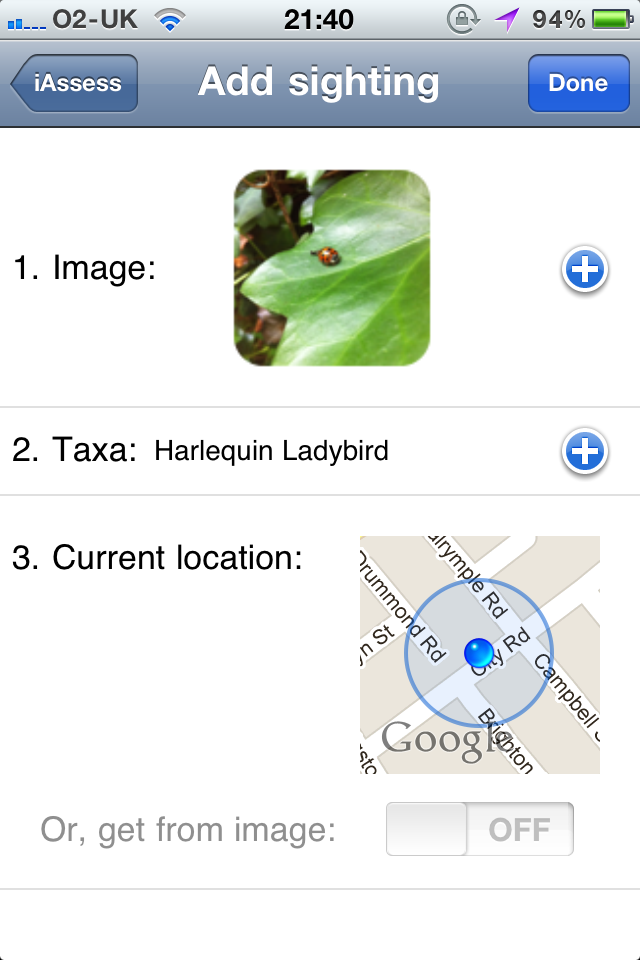
\includegraphics[width = 5cm]{img/iAssess.png} % requires the graphicx package
   \caption{iAssess iPhone app.}
   \label{fig:iOS}
\end{figure}

\emph{Scientists attempting to establish the effects of IAS need technology to assist - can survey large areas to locate certain species and apply sampling methods (e.g. Jones et al) but not for species like Harmonia, which are fast spreading. Technology has to compete with the speed of spread.}

\section*{\fontfamily{phv}\selectfont{\normalsize{\bfseries{Management}}}}

\emph{In terms of control, management strategies need to consider not only locations but also properties of the species cohort -- size may affect ability to manage quickly, and discovery of different levels of invasion allow for better management plan....
}

\section*{\fontfamily{phv}\selectfont{\normalsize{\bfseries{Conclusion}}}}

\bibliographystyle{agsm}
\addtolength{\bibsep}{-2mm}
{\footnotesize
\bibliography{papers}}
\end{document}
